\documentclass[10pt,twocolumn,letterpaper]{article}

\usepackage{cvpr}
\usepackage{times}
\usepackage{epsfig}
\usepackage{graphicx}
\usepackage{subcaption}
\usepackage{amsmath}
\usepackage{amssymb}
\usepackage{dsfont}
\usepackage{bm}
\usepackage{bbm}
\usepackage{amsfonts,amscd}
\usepackage{amssymb,amsmath,amsthm,enumerate}
\usepackage{physics}

\usepackage{tikz}
\usetikzlibrary{calc}
\usetikzlibrary{shapes,arrows}

\usepackage{algorithm}
\usepackage{algpseudocode}  % including algorithms

\DeclareMathOperator*{\argmax}{arg\,max}
\DeclareMathOperator*{\argmin}{arg\,min}

% Include other packages here, before hyperref.

% If you comment hyperref and then uncomment it, you should delete
% egpaper.aux before re-running latex.  (Or just hit 'q' on the first latex
% run, let it finish, and you should be clear).
\usepackage[breaklinks=true,bookmarks=false]{hyperref}

\cvprfinalcopy % *** Uncomment this line for the final submission

\def\cvprPaperID{****} % *** Enter the CVPR Paper ID here
\def\httilde{\mbox{\tt\raisebox{-.5ex}{\symbol{126}}}}

% Pages are numbered in submission mode, and unnumbered in camera-ready
%\ifcvprfinal\pagestyle{empty}\fi
\setcounter{page}{1}
\begin{document}

%%%%%%%%% TITLE
\title{Continuous Control in Bearing-only Localization}

\author{
  Cedrick Argueta \\
  \texttt{cedrick@cs.stanford.edu} \\
}

\maketitle
%\thispagestyle{empty}

%%%%%%%%% ABSTRACT
\begin{abstract}
In this work we model localization in the context of source seeking with drones.
Specifically, we show how an autonomous drone fitted with radio antennas can minimize uncertainty over belief of a radio target.
We model the problem as a belief Markov decision process and use deep deterministic policy gradient and twin delayed deep deterministic policy gradient as controllers.
\end{abstract}

\section{Introduction}
Tracking a moving radio target is useful in a variety of situations.
An unauthorized drone could be disrupting airport operations, causing delays, or interfering with aircraft.
A wildlife radio tag could help with studying migration patterns of migrant animals.
Sophisticated control is often necessary in localization -- sensors are often noisy and it's difficult to encode priors on the target's movement in some situations.
In addition to localization, we study the added constraint of avoiding near collisions with the target: e.g. a drone tracking a wildebeest should not get so close that it frightens the animal.
The introduction of a near collision penalty is what makes this problem interesting: the optimal policy is often a balance between information gather actions (getting close to the target to receive better observations) and respecting the collision penalty.
In this work, we model this problem as a dynamic system and apply two continuous control algorithms, deep deterministic policy gradient (DDPG) \cite{ddpg} and twin delayed DDPG (TD3) \cite{td3} as solution methods.
These methods are compared to deep Q-learning (DQN) \cite{dqn} and a greedy method as baselines.
We show that continuous learning-based methods improve on a greedy baseline in terms of localization quality and collision rate, however, further work must be done to show that continuous control dominates discrete control.

\section{Related Work}
This work primarily builds off of work done on efficient, low-cost localization with drones.
Drones have been used in localization because of their ease of use and mobility \cite{dronehunter}, \cite{kyle1}, \cite{learning_to_seek}.
Particle filters in localization and modeling tasks are explored in \cite{dronehunter} and \cite{kyle1}.
Traditional control with a receding horizon controller is compared with reinforcement learning in \cite{kyle1}, while \cite{dronehunter} compares a greedy controller with Monte Carlo tree search.
We base our dynamics models on those in \cite{dronehunter} and take cues on learning algorithms for control from \cite{kyle1}.

The sensor model used in this work is based off of \cite{sensor_modality}, which describes how antennas may be used to generate bearing measurements relative to a drone.
While sensing is not the primary aim of this paper, it is prudent to note that the sensor choice often dictates the difficulty of localization.
Other works demonstrate localization with sensors that are easier to implement in practice but yield lower information that the sensor used in this work \cite{fov}.


\section{Mathematical Models}
\label{sec:models}

\subsection{Drone Dynamics}
We assume that the target is another drone, so the major components of our environment are a seeker drone and a target drone.
The drone dynamics are exactly those described in \cite{dronehunter}.
The seeker drone state at time $t$ is $x_t = [x_t^n, x_t^e, x_t^h]^\intercal$, where $x_t^n$ and $x_t^e$ are the seeker's north and east coordinates and $x_t^h$ is the seeker's heading measured east of north.
The state described here does not contain velocity or altitude as simplifying assumptions.
The drone follows a first-order motion model, so the state after applying a control input $u_t$ for duration $\Delta t$ the new state is
\begin{equation}
x_{t + \Delta t} = x_t + u_t\Delta t
\end{equation}

The target drone state at time $t$ is $\theta_t = [\theta_t^n, \theta_t^e]^\intercal$, where $\theta_t^n$ and $\theta_t^e$ are the target's north and east coordinates.
The target drone is assumed to move with a constant velocity $\dot{\theta} = [\dot{\theta_t^n}, \dot{\theta_t^e}]^\intercal$.
The drone follows a first-order motion model, so the state after $\Delta t$ is
\begin{equation}
\theta_{t + \Delta t} = \theta_t + \dot{\theta_t}\Delta t
\label{target_dynamics}
\end{equation}

\subsection{Sensor Model}
The bearing from the seeker drone to the target drone is 
\begin{equation}
\beta_t = \arctan{\frac{\theta_t^e - x_t^e}{\theta_t^n - x_t^n}}
\end{equation}
when measured east of north.
Configured properly, a directional antenna and omnidirectional antenna can give estimates of the relative bearing of the target drone.
 \cite{sensor_modality}

At time $t$, the seeker drone makes measurement $z_t \sim \mathcal{N}(\beta_t - x_t^h, \sigma^2)$, which is a bearing in the interval $[0^{\circ}, 360^{\circ}]$.
It is assumed that these measurements are normally distributed about the true relative bearing with some variance to account for sensor error.
In this work, the standard deviation of the sensor measurements is assumed to be $5^{\circ}$.

\subsection{Particle Filter}
The seeker drone maintains a belief of the possible location of the target drone, which is modeled with a particle filter \cite{decision_making}, \cite{prob_rob}.
It is useful to think of a particle filter as a type of hidden Markov model: as evidence from the sensor is received, we can update our belief of the true state of the system.
Belief at time $t$ is represented by a set $b_t$ of $N$ particles, each representing a hypothesis of the target drone's pose.
Updates are made to the particle filter at every timestep to improve the belief's accuracy.

The belief update consists of three steps. 
The first step is the prediction step, where each particle is propagated according to the dynamics described in equation \ref{target_dynamics}.
Noise is added to the dynamics to prevent particle deprivation, a situation that arises when all particles converge to a hypothesis that doesn't accurately represent the true state.
The second step is the weighting step, where each particle is assigned a weight according to how probable an observation $z_t$ is given the particle's position.
The third step is resampling, where particles are sampled according to these weights with replacement.
In this work, we use stratified resampling to aid in maintaining an accurate estimate of the target while ensuring resiliency to particle deprivation.

In planning, $\mathbb{E}\left [ b_t \right ]$ is used by the controller. 
Namely, this provides the controller with the estimate of $\theta_t$ and $\dot{\theta_t}$.
With the mean of the particle filter, we are effectively performing feature engineering -- rather than directly use the relative bearing provided by the sensor, we construct a particle filter and use the estimates instead.
This helps to cut down on the noise introduced by inaccuracies in the sensor model, alleviating some of the stochasticity that the learning algorithm must deal with.

\subsection{Belief Markov decision process}

\subsubsection{States}
The problem described is actually a partially observable Markov decision process (POMDP), as the agent cannot fully observe the environment at each step $t$.
Since it is difficult to incorporate a belief-dependent reward (such as entropy minimization) into a POMDP, we hereafter model the problem as a belief MDP where each state is a tuple of the fully observable part of the true state (seeker position) and the belief of the partially observable part of the true state (estimate of target position and velocity from the particle filter) \cite{dronehunter}.
In our analysis, each state is a tuple $s_t = (x_t, b_t)$.
However, our controller makes a simplification and uses the mean estimate of the particle filter for states, so the controller actually uses $s_t = (x_t, \hat{\theta_t}, \hat{\dot{\theta_t}})$.

\subsubsection{Actions}
In the discrete setting used for the greedy and DQN controllers, the seeker drone travels with constant velocity in one of 12 directions spaced radially about the seeker drone, effectively allowing the seeker to choose any multiple of $30^{\circ}$ as a heading.
In the continuous setting used for the DDPG and TD3 controllers, the seeker drone must instead choose a heading to travel towards, with a full $360^{\circ}$ range of motion.

\subsubsection{Reward Function}
Our reward function for radiolocation captures the desire to maintain an accurate and precise estimate of the target's location \textit{while also} maintaining an acceptable distance from the target.

A precise belief is one that has low uncertainty over the target's position.
Minimization of this uncertainty is equivalent to minimization of the entropy of the belief distribution.
Particles in the filter are first discretized into $M$ bins.
Entropy can then be defined as:
\begin{equation}
H(b_t) = -\sum_{i = 1}^M\tilde{b}_t[i]\log\tilde{b}_t[i]
\label{entropy_unnormalized}
\end{equation}
where $\tilde{b}_t$ is the proportion of particles in each bin.

Near-collisions are penalized to encourage the seeker to keep a safe distance.
The penalty term contains only the belief of the belief of the target's position rather than the true target position.
This is to encourage the seeker to maintain a distance from the particles during evaluation.
If the belief is representative of the true state, then the seeker will maintain a safe distance.
If the belief is not representative of the true state, then the seeker will at least maintain a distance from the belief, which still might contain a noisy or partially accurate model of the target's motion.
Our near-collision penalty is
\begin{equation}
C(b_t, x_t) = \mathop{{}\mathbb{E}}_{b_t} \mathds{1} (\Vert x_t - \hat{\theta_t}\Vert < d)
\label{collision_penalty}
\end{equation}
where $\mathds{1}$ is an indicator function and $d$ is the safe distance we wish the seeker to maintain.
In this work, $d = 15m$.

The terms are combined to produce our full reward function:
\begin{equation}
R(s_t) = H(b_t) - \lambda C(b_t, x_t)
\label{reward_function}
\end{equation}
where $\lambda$ is a coefficient controlling the tradeoff between entropy minimization and collision avoidance.
In this work, $\lambda = 1$.

\section{Methods}

\subsection{DDPG}
DDPG is an off-policy reinforcement learning algorithm for use with continuous action spaces \cite{ddpg}.
The algorithm is detailed in algorithm \ref{alg:ddpg}.

The algorithm works by maintaining an actor function and critic function, both approximated by neural networks.
The actor function receives as input the state of the environment, and outputs an action in the continuous action space.
The critic function receives as input the state of the environment and the action taken at that time, and outputs the expected value attained from taking that transition.
By minimizing the mean squared error between each $y_i$ and output of $Q$, we approximate the $Q$ value function.
The actor function is optimized directly to output actions that maximize expected return.

A variety of modifications were needed to make DDPG a viable solution method in the context of deep reinforcement learning.
First, an experience buffer is needed to minimize correlations between samples.
Second, target networks are required to stabilize learning.
Both of these modifications were introduced in \cite{dqn}, where the popular Q-learning algorithm \cite{sutton_barto_2018} was modified with neural networks to play Atari video games.


\begin{algorithm}
\caption{Deep Deterministic Policy Gradient}
\label{alg:ddpg}
\begin{algorithmic}[1]
\State Initialize replay memory $\mathcal{D}$
\State Initialize actor network $\mu$ and critic network $Q$
\State Initialize target networks $\mu'$ and $Q'$
\For{$\textrm{episode} = 1, M$}
    \State Initialize sequence $s_1$ 
    \State Initialize random process $\mathcal{N}$ for exploration
    \For{$t = 1, T$}
        \State Select action $a_t = \mu(s_t) + \mathcal{N}_t$
        \State Execute action $a_t$ and observe reward $r_t$ and observe new state $s_{t+1}$
        \State Store transition $(s_t, a_t, r_t, s_{t+1})$ in $\mathcal{D}$

        \State Sample random minibatch of $N$ transitions $(s_i, a_i, r_i, s_{i + 1})$
        \State Set $ \displaystyle  y_i = r_i + \gamma Q'(s_{i + 1}, \mu'(s_{i + 1}))$
        \State Update critic by minimizing loss equal to MSE of $y_i = Q(s_i, a_i)$
        \State Update actor with policy gradient $ \displaystyle \nabla J \approx \frac{1}{N} \sum_{i} \nabla_{a}Q(s, a) \nabla \mu(s) $

        \State Update target networks
    \EndFor
\EndFor
\end{algorithmic}
\end{algorithm}




\subsection{TD3}
Twin delayed deep deterministic policy gradient (TD3) proposes further modifications to the original DDPG algorithm to improve stability and improve learning \cite{td3}.
Three main improvements are proposed.

\subsubsection{Twin $Q$ networks}
In an improvement to DQN, \cite{double_dqn} implements a variant of the DQN update that reduces overestimation common to value function methods.
Such an update in DDPG is difficult to use because the update will then use the current policy rather than the target policy in each $y_i$.
Instead, a second target $Q$ network is used.
Each learning target then becomes $\displaystyle y_i = r_i + \gamma \min_{j=1, 2}{{Q'}_j(s_{i + 1}, \mu'(s_{i + 1}))}$.
The minimum here promotes underestimation of the value function, which is preferable to overestimation.

\subsubsection{Delayed Policy Updates}
The second improvement is a delay in updates for the actor network and target networks.
The goal of this modification is to improve the gradient steps taken by the policy during updates.
The actor is then updated against a critic with lower variance, as more critic updates occur compared to the actor.
In practice, the actor is updated once for every two critic updates.

\subsubsection{Target Policy Smoothing}
The final improvement is with the learning targets themselves.
The authors aim to fit the value function around a region of actions rather than a deterministic action. 
The reasoning here is that inaccurate value function approximation may include peaks or dips in the area around a particular action, resulting in wildly different value estimates for similar actions.
Adding a smoothing factor to the updates in the form of random noise combats this by enforcing similar value function estimates for similar actions.
Then the learning update becomes $\displaystyle y_i = r_i + \gamma \min_{j=1, 2}{{Q'}_j(s_{i + 1}, \mu'(s_{i+1}) + \epsilon)}$, where $\epsilon \sim clip(\mathcal{N}(0, 0.2), -0.5, 0.5)$.



\section{Results}


\subsection{Experimental Setup}
Experiments were performed using the open source drone simulation package PyFEBOL \cite{PyFEBOL}.
The seeker and target drones live inside a $200m \times 200m$ area.
To best describe the target drone placement, imagine that there is a $180m \times 180m$ box within the search environment, centered such that there is $10m$ of space all around the smaller square.
The target drone starts at a random corner of this smaller square and follows an edge to an adjacent corner at a speed of $1.7\frac{m}{s}$.
The seeker drone starts each episode at the center of the search area, and can move at $5\frac{m}{s}$.
Each episode runs for 100 steps, giving ample time for the seeker drone to catch the target drone and accumulate rewards.

The particle filter used to model the environment has $2000$ particles and is discretized into a $50 \times 50$ matrix for entropy calculation.
It is important to note that the particle filter is necessarily stochastic, as noise is added during particle prediction so that the filter does not degenerate to a single particle.
This stochasticity is difficult for the controllers to handle -- it's possible that a controller takes a `good' action but doesn't receive a matching good reward, as the particle filter just so happened to concentrate belief in a different way.
This stochasticity works itself out in expectation, but in real systems this affects the sample efficiency of our learning algorithms greatly.

Hyperparameters for the learning algorithms used are available in table \ref{hyperparams}.
All training was performed on a Google Cloud Platform virtual machine with 15 GB of RAM and an Nvidia Tesla K80 GPU.
Batch size was chosen to maximize usage of the GPU, while memory size was chosen to maximize RAM usage.
Learning rate was chosen emprically, where the chosen rate was the best performing out of all rates tried.
All neural networks used had a very similar structure.
Actor networks used $s_t$ for input (7 floats: seeker position and heading, estimated position of target, estimated velocity of target) and were followed by two hidden layers of size 512 and 384 with ReLU activations.
Critic networks were very similar, but appended the action taken (1 float: heading) to the input layer.
Output depended on the function to be approximated: critic networks had the raw values of the neural network as output, while actor networks used a Tanh activation function to scale output between [$-1, -1$].


\subsection{Metrics}

\subsubsection{Tracking Error}
Tracking error is defined as $\Vert \theta_t - \hat{\theta_t}\Vert$.
It is the error that the particle filter has with respect to target position.
Tracking error is included as a more intuitive measure of filter accuracy than nats of entropy.
It is easier to interpret a tracking error of $5m$ than an entropy of $3.0$ nats.

\subsubsection{Collision Rate}
As per our reward function in equation \ref{reward_function}, we seek to minimize the probability of near collisions with our controller.
The collision rate is the percentage of the episode that the seeker is within collision distance of the target.

\subsubsection{Average Cost}
The cost represented in equation \ref{reward_function}, averaged over all steps in the episode.
Depending on the value of $\lambda$, the optimal policy will change to maximize different objectives.
If $\lambda = 0$, then the optimal policy is for the seeker drone to hover over the target drone, minimizing entropy as much as possible with no regard to near collisions.
Why is it optimal to minimize distance to the target drone when sensor accuracy is the same at all distances?
This is because the information gathered closer to the target is greater: the parallax subtended by the target drone moving with respect to the seeker drone is larger when the seeker is closer to the target.
The filter is then more likely to update to a better representation of the true state.
If $\lambda$ becomes large, it is optimal to avoid all particles so that no cost is incurred by the near collision penalty.
In this case, localization is still possible, as the seeker may circle the target from afar and concentrate belief relatively well.

\begin{table}[]
\begin{tabular}{|l|l|l|l|l|}
\hline
     & batch size & memory size & learning rate & target update \\ \hline
DQN  & 128        & 100000      & 0.0005        & 0.0005        \\ \hline
DDPG & 128        & 100000      & 0.001         & 0.001         \\ \hline
TD3  & 128        & 100000      & 0.001         & 0.001         \\ \hline
\end{tabular}

\begin{tabular}{|l|l|l|l|l|}
\hline
     & warmup steps & eps\_start & eps\_end & eps\_decay \\ \hline
DQN  & 1000         & 0.9            & 0.1          & 1666           \\ \hline
DDPG & 10000        & 0.9            & 0.1          & 1666           \\ \hline
TD3  & 10000        & 0.9            & 0.1          & 1666           \\ \hline
\end{tabular}
\caption{Hyperparameters used during training.}
\label{hyperparams}
\end{table}


\subsection{Comparison of Controllers}

\subsubsection{Greedy}
The greedy method iterates over all possible actions and chooses that which maximizes the reward function for that step.
Since it takes the lowest cost action at every step, it never plans ahead to incur some penalty to get close to the target and then receive a much higher reward.
The greedy solver only maintains a filter with a tracking error of greater than $30m$, which may or may not be suitable given the task.
This error might be acceptable when tracking a highly erratic animal, but less so when tracking a car with constant velocity on a highway.


\subsubsection{DQN}
The second controller is the standard DQN algorithm, which makes Q-learning tractable with continuous observation spaces through the use of neural networks.
The DQN controller is trained until convergence, which happens after about 1800 episodes across all random seeds used.
It's interesting to note that the DQN controller is very susceptible to catastrophic forgetting, where some time after convergence performance degrades significantly.
Despite this, the DQN controller performs fabulously, learning that the long-term reward from incurring the collision penalty is greatly outweighed by reduction in entropy. 
This also validates our choice of state space, showing that learning the optimal policy with mean estimates from the particle filter is possible.
This controller reveals that the optimal policy is to disregard the collision rate, as with $\lambda = 1$ the cost of collisions is greatly outweighed by the reward from entropy reduction.
This can be seen in figure \ref{fig:compare}.

\subsection{DDPG and TD3}
The continuous controller presents an interesting yet suboptimal policy.
The controller learns to avoid all particles and observe from afar.
The effective collision rate is 0, because as soon as belief is updated after the first step the controller takes actions to move away from the concentrated belief.

An interesting degenerate behavior of the particle filter appears both in the greedy case and with the continuous controllers.
When the seeker is farther away from the target, many actions must be taken to receive the same information than when the seeker is close to the target.
Again, this is due to the information gained from parallax.
An illustrative case can be seen in figure \ref{fig:compare}, where the belief is concentrated in a line from the seeker to the target.
The controller's optimal action would be to move to the orthogonal axis of the belief distribution, yet the controller fails to learn this behavior.

Despite similar behavior to the greedy method, continuous control is not a total failure, as it still dominates the greedy method in all performance metrics.
Tracking error, while still significantly larger than that of DQN, is further reduced in TD3. 
This indicates that despite maintaining a similar collision rate and average entropy to DDPG, TD3 manages to take actions that improve the particle filter's accuracy rather than precision.



\begin{table}[]
\begin{tabular}{|l|l|l|l|}
\hline
       & Tracking Error & Collision Rate & Average Cost \\ \hline
Greedy & $30.5m$        & 1.8\%          & -4.18        \\ \hline
DQN    & $5.4m$         & 62\%           & -2.37        \\ \hline
DDPG   & $20.1m$        & 0\%            & -3.73        \\ \hline
TD3    & $13.5m$        & 0\%            & -3.75        \\ \hline
\end{tabular}
\caption{Performance of controllers against three different metrics, averaged over 100 episodes.}
\label{results}
\end{table}




\begin{figure}[h!]
  \centering
  \begin{subfigure}[b]{0.48\linewidth}
    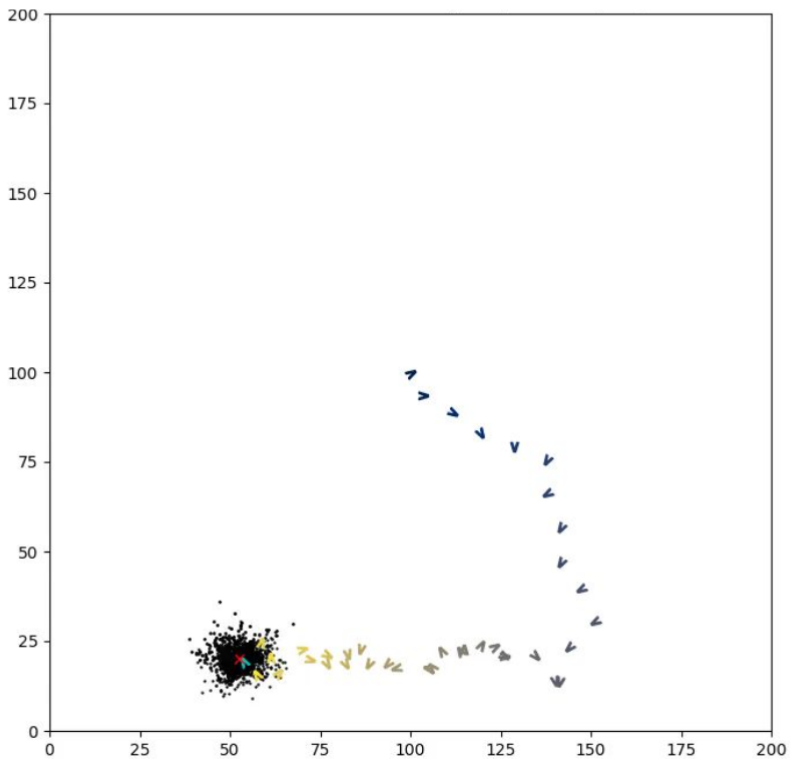
\includegraphics[width=\linewidth]{images/dqn-policy.png}
    \caption{Policy learned by DQN.}
  \end{subfigure}
  \begin{subfigure}[b]{0.48\linewidth}
    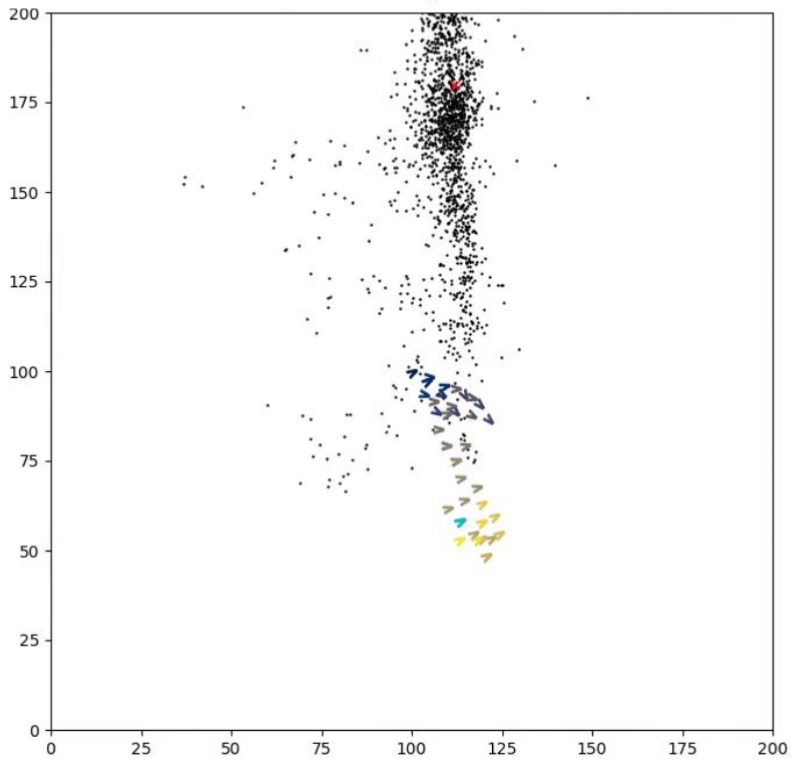
\includegraphics[width=\linewidth]{images/td3-policy.png}
    \caption{Policy learned by TD3.}
  \end{subfigure}
    \caption{The brighter chevrons indicate more recent positions of the seeker, the black dots are particles in the filter, and the red x is the target.}
  \label{fig:compare}
\end{figure}


\section{Conclusion and Future Work}
In conclusion, we show that continuous learning-based methods improve on a greedy baseline in terms of localization quality and collision rate, however, further work must be done to show that continuous control dominates discrete control.
Discrete control through DQN proved victorious in these experiments.
It's likely that some performance gain would have been possible with the continuous control algorithms if we had more time -- training DDPG and TD3 took significantly longer than DQN.
Because the limiting factor was training time, leveraging techniques like asynchronous updates \cite{a3c} or learning from demonstrations \cite{dqfd} may have allowed for more time to perform hyperparameter search or may have improved model stability.

\subsection{Particle Filter}
Instead of taking the mean of the particle filter for estimating the state, it is possible to use the whole particle filter \cite{dronehunter}, \cite{kyle1}.
Particle filters are often highly non-Gaussian, so a simple mean and standard deviation does not accurately represent the distribution.
Fine discretization can turn a particle filter into a 2D grid, which can be passed to a convolutional neural network for learning algorithms.
This may result in higher quality inference, particularly with more interesting target motion models.

\subsection{Model-based Reinforcement Learning}
The particle filter can be interpreted as a form of feature engineering, where we construct the filter based on the relative bearing measurement given to us by the antenna.
However, we lose the particle filter after every episode and must construct it again from scratch because we begin in a new environment possibly unlike the previous one.
Is there a way to leverage the particle filter across training to improve sample efficiency through model-based reinforcement learning?

\subsection{Flight Tests}
The PyFEBOL drone simulation package and experiments run in this paper correspond to a set of experiments that were run in SISL.
It would be interesting to demonstrate some of these learned policies on an actual drone!


\section{Contributions}
I worked on this project alone.

{\small
\bibliographystyle{unsrt}
\bibliography{ref}
}

\end{document}
